\documentclass[a4paper,12pt]{article}
\usepackage[a4paper, margin=2.4cm]{geometry}
\usepackage[utf8]{inputenc}
\usepackage{amsmath, amssymb} % Packages pour les maths
\usepackage[T1]{fontenc}
\usepackage{graphicx} 
\usepackage{caption}
\usepackage{setspace} % Espacement des lignes
\usepackage{tikz}
\begin{document}
\section{Modèle 1:}
\subsection{Bille remplie d'eau}
\textbf{Hypothèses}:
\begin{itemize}
    \item Terre assimilé à boule d'eau, de température \(T_{\text{Terre}}\) telle que \(T_{\text{Terre}}\)> \(T_{\text{vide}}\)
    \item  Sans atmosphère (dans le vide)
    \item  Sans puissance solaire reçue  
    \item \(C= C_{\text{eau}} \sim C_{\text{terre}}\) 
    \item $T(t=0) = T_i$ \ \ \
$T(t \to +\infty) = T_0$
   
\end{itemize}
$\rightarrow$ la terre perd de la température par rayonnement
\textbf{Equations :} 
\[   P= \sigma T^4 
\]

\[    C \, \frac{dT}{dt} = - \sigma T^4 \, dt \times S
\]

\[\frac{dT}{dt} = - \frac{4 \pi R_T^2 \sigma T^4}{C}\]  

\textbf{Solution:} 
\[
T(t) = \left( \frac{C}{C/T_i^3 + 12\pi R^2 \sigma t} \right)^{1/3} 
= \frac{T_i}{\left(1 + 3k T_i^3 t \right)^{1/3}}
\]
avec \(k=\frac{4\pi R_T^2 \sigma}{C}\)
et \(C=c_{\text{m eau}}\times m=4,60 \cdot 10^{27} J\cdot K^{-1}\)

\bigskip



\bigskip
\textbf{Modélisation:} 
    
    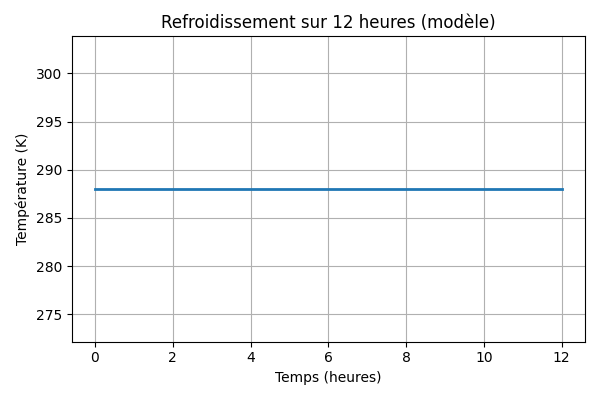
\includegraphics[width=0.8\linewidth]{../modele1/figures/modele1.png}
\\
\subsection{Coquille vide }
\textbf{Hypothèses}:
\begin{itemize}
    \item Terre assimilée à une coquille d'eau, d'épaisseur dr, avec du vide à l'intérieur
    
\end{itemize}
$\rightarrow$ il faut donc recalculer la capacitée thermique 


\begin{align*}
m &= \rho_{\text{eau}} \left( \frac{4}{3} \pi (R_T + dr)^3 - \frac{4}{3} \pi R_T^3 \right) \\
&\overset{DL}{\approx} \rho_{\text{eau}} \cdot 4\pi R_T^2 \cdot dr \\
\\
C &= c_{\text{eau}} \cdot \rho_{\text{eau}} \cdot 4\pi R_T^2 \cdot dr \\
&= 4{,}31 \cdot 10^{20} \ \text{J} \cdot \text{K}^{-1} \\
\\
k &= \frac{4\pi h }{c_{\text{eau}} \cdot \rho_{\text{eau}} \cdot 4\pi R^2 \cdot dr}
\end{align*}

    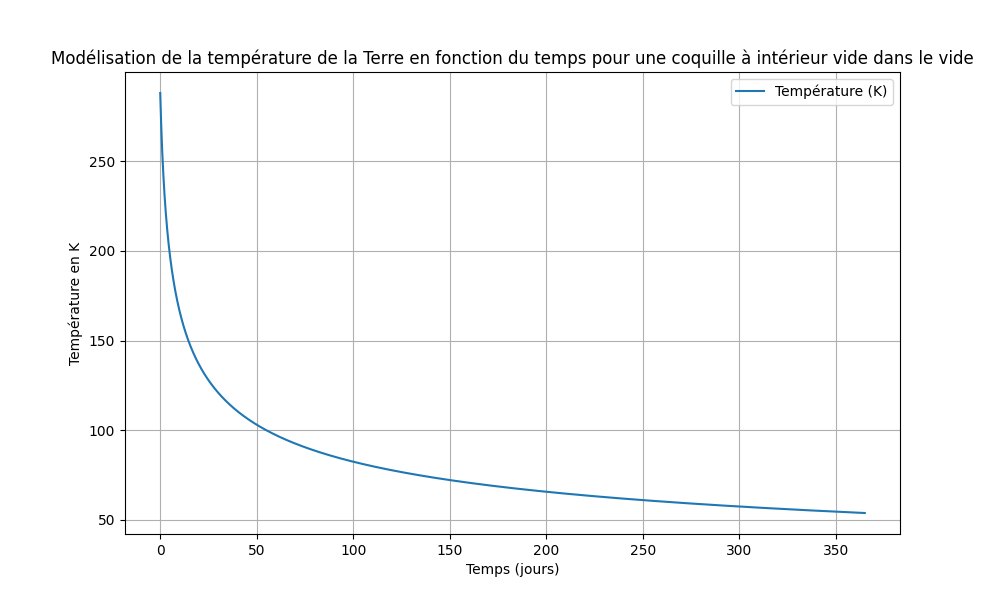
\includegraphics[width=0.8\linewidth]{../modele1/figures/modele1_coquille.png} 

\end{document}